\chapter{\IfLanguageName{dutch}{Stand van zaken}{State of the art}}
\label{ch:stand-van-zaken}

%%=============================================================================
%% Selectie van bronnen
%%=============================================================================
\section{Selectie van bronnen}
\label{sec:selectie-van-bronnen}
Om deze literatuurstudie en deze bachelorproef an sich als volwaardig en kwalitatief te kunnen aanschouwen volgt eerst een kleine uitleg rond de keuze voor ondersteunende bronnen.
De selectiecriteria bouwt hierbij verder op de CRAAP-test, opgesteld door~\textcite{Blakeslee2004}.

%---------- Uitleg CRAAP-test ----------------------------------------------------------
\subsection{De CRAAP-test}
\label{subsec:de-craap-test}
De CRAAP-test bestaat uit volgende criteria, zoals gezien in de syllabus IT-component van het opleidingsonderdeel Research Methods~\autocite{Bert2023}:
\begin{itemize}
    \item \textbf{Currency} of actualiteit: de aangehaalde bron is recent genoeg voor het onderwerp.
    \item \textbf{Relevance} of relevantie: het doelpubliek van de bron past bij het doelpubliek van deze paper, bovendien past de geciteerde inhoud bij de literatuurstudie.
    \item \textbf{Authority} of autoriteit: er is geen mogelijke belangenconflict van de auteur van de bron.
    De auteur heeft eveneens een gepaste achtergrond als vakexpert of is verbonden met een betrouwbare instantie.
    \item \textbf{Accuracy} of correctheid: de bron werd onderwerpen aan een peer review-proces, heeft zelf verifieerbare bronnen of resultaten en heeft genoeg diepgang.
    \item \textbf{Purpose} of doel: het doel van de auteur is om een volwaardige tekst te schrijven zonder vertekend beeld.
    Hierbij is duidelijk of de inhoud gaat over een mening of over feiten, tevens sluit het doel van de bron aan bij het doel van deze paper.
\end{itemize}

%---------- Zoekstrategieen ------------------------------------------------------------
\subsection{Gebruikte zoekstrategiëen}
\label{subsec:zoekstrategieen}
Zoekmachines en publicatieplatformen zoals Google Scholar en ResearchGate maken het mogelijk om allerlei publicaties te vinden rond het gepaste onderwerp.
Artifici\"eele intelligentie kent een voortdurend proces van verbeteringen vergelijkbaar met het agile werken in de rest van de softwareontwikkelingsindustrie.
Hierdoor is het belangrijk dat bronnen ge\"evalueerd worden volgens hun actualiteit.
De focus ligt hierdoor op bronnen die de afgelopen 3 jaar gepubliceerd werden, tevens wordt gekeken of de inhoud nog actueel is aan recentere ontwikkelingen.
Een uitzondering wordt gemaakt voor onderzoeken over lang bestaande onderwerpen waarvan de inhoud niet vaak zal veranderen, in het bijzonder klassieke objectherkenningsalgoritmen.
Bronnen dienen eveneens relevant te zijn aan deze paper, daarvoor wordt gekozen voor bronnen waarvan het onderwerp overeenstemt met artifici\"ele intelligentie.

%---------- Selectiecriteria -----------------------------------------------------------
\subsection{Selectiecriteria}
\label{subsec:selectiecriteria}
Na het filteren van irrelevante en verouderde bronnen komt het beoordelen van de autoriteit en het doel van de bron aan bod.
Waar mogelijk is de bron geschreven met als doel om aan een conferentie of universitaire colleges voor te dragen.
Eveneens zijn bronnen die gepubliceerd werden in een betrouwbare wetenschappelijk tijdschrift aanvaardbaar.
Een wetenschappelijke tijdschrift kan als betrouwbaar aanschouwd worden als publicaties door vakgenoten beoordeeld worden.
Tevens worden ook bronnen die reproduceerbaar zijn als geldige, betrouwbare aanschouwd.

%---------- Bronnen buiten literatuurstudie---------------------------------------------
\subsection{Bronnen buiten de literatuurstudie}
\label{subsec:bronnen-buiten-de-literatuurstudie}
Bij het opstellen van de shortlist met gebruikte technologie\"en en het uitwerken van de proof-of-concept zal er voornamelijk naar technische bronnen verwezen worden, dit in tegenstelling tot de academische bronnen die in deze literatuurstudie aangehaald worden.
De bovenstaande selectiecriteria zijn hierbij ook van toepassing, met de uitzondering dat er gekeken zal worden naar documentatie van vertrouwde omgevingen in plaats van wetenschappelijke tijdschriften.
Een omgeving is vertrouwd als het gaat om een bewezen ecosysteem met actieve ontwikkelaars en stabiel genoeg is om in productie genomen te worden.

%%=============================================================================
%% Klassieke objectherkenning
%%=============================================================================
\section{Klassieke objectherkenning}\label{sec:ls-object-detectie}
Omdat objectdetectie de kern van de proof-of-concept zal vormen, is het van essentieel belang om eerst een grondig begrip te defini\"eren van wat deze techniek precies inhoudt.
In dit hoofdstuk zal eerst computer visie aan bod komen, een van de gebieden van hedendaagse artifici\"ele intelligentie, waarbinnen objectherkenning zich plaats vindt.
Dit zal verduidelijkt worden aan de hand van enkele praktische toepassingen die vandaag al in gebruik genomen worden met behulp van computer visie en objectherkenning.
Daarna volgt een uitleg van de processen waarop beelden opgeslagen en verwerkt worden ter voorbereiding op het toepassen van objectherkenning.
Vervolgens worden enkele traditionele objectdetectie algoritmen besproken die de verwerkte data kunnen interpreteren.
Tot slot komen enkele uitdagingen en limitaties van klassieke algoritmen aan bod, waar het volgende hoofdstuk een mogelijk antwoord op kan bieden.

%---------- Computervisie --------------------------------------------------------------
\subsection{Computer visie}\label{subsec:de-kern-van-objectdetectie}
Computer visie is een van de vele vakgebieden binnen de kunstmatige intelligentie en richt zich op het interpreteren van multimedia~\autocite{Moin2023}.
Met de komst van dit vakgebied ontstaat een grote waaier aan mogelijkheden voor computers om bij te staan bij complexere taken zoals gezichts- en emotieherkenning, sc\`eneanalyse en objectherkenning.
Hiermee beschrijven~\textcite{Tasnim2023} dat objectdetectie een fundamentele taak omvat binnen dit vakgebied waarmee het identificeren en lokaliseren van objecten mogelijk wordt op (bewegende) beelden.
De ontwikkelingen in dit vakgebied worden vandaag steeds meer gebruikt in allerlei sectoren:

\subsubsection{Computer visie in de landbouwsector}
\textcite{Radojcic2023}~beschrijven in zijn conferentiepaper voor de 15de Internationale Landbouwsymposium `AGROSYM 2023' conferentie het volgende over computer visie in de landbouw:
``De integratie van robotica, slimme landbouw en computervisietechnologie\"en in de landbouw heeft een transformerende verschuiving in de industrie teweeggebracht.
Het gebruik van computervisiealgoritmen heeft een cruciale rol gespeeld in het realtime monitoren en beheren van gewassen.
Door afbeeldingen en video's te analyseren, bieden deze algoritmen boeren tijdige en nauwkeurige informatie over de groei en ontwikkeling van hun gewassen, waardoor ze ge\"{\i}nformeerde beslissingen kunnen nemen over bemesting, irrigatie en pesticidegebruik.''
Deze resultaten binnen de landbouwsector worden gerealiseerd door middel van objectherkenning binnen computervisie.
Om het gebruik hiervan mogelijk te maken worden deep learning algoritmes zoals convolutionele neurale netwerken (CNN) toegepast, meer hiervan komt aan bod in het hoofdstuk~\nameref{sec:datasets}.

\subsubsection{Computer visie in zelfrijdende auto's}
Een tweede voorbeeld is het toepassen van computer visie in de transportsector.
Met behulp van computer visie-algoritmen zoals kleurenruimte transformatie, Canny-randdetectie en Hough-lijntransformatie wordt het mogelijk voor zelfrijdende auto's om op een goedkopere wijze berekeningen te maken~\autocite{Gajjar2023}.
Door middel van deze algoritmen verdwijnt de noodzaak om te ondersteunen op duurdere systemen, met name Lichtdetectie- en afstandmetingssensoren (LiDAR) die gebruikt worden om een virtuele driedimensionele map te maken van de direct omgeving.
Beide systemen kennen een vorm van objectherkenning om objecten zoals verkeersborden of voertuigen in de omgeving te detecteren, een visualisatie van het LiDAR-systeem in zelfrijdende auto's is terug te vinden op afbeelding~\ref{fig:visualisatie-lidar}.
De implementatie hiervan kent echter de moeilijkheid van data-analyse in donkere momenten zoals na zonsondergang, waardoor de kwaliteit van binnenkomende data afzwakt door het lage licht.
Een mogelijke oplossing hierbij is het toevoegen van infrarood lampen gecombineerd met een infraroodcamera.
Ook hierbij wordt het mogelijk om via CNN-algoritmes te bepalen wanneer overgestapt moet worden op een alternatief systeem.
\begin{figure}
    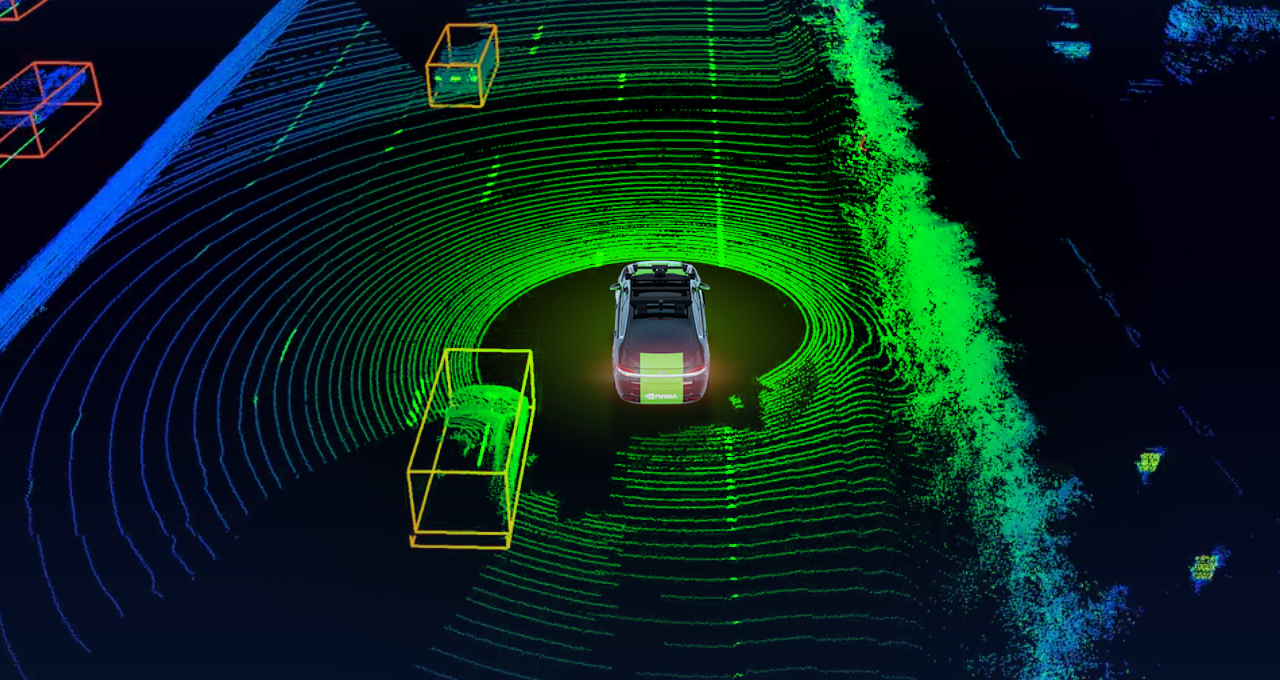
\includegraphics[scale=0.35]{images/visualisatie-lidar}
    \caption{Visualisatie van een LiDAR-systeem met objectherkenning in auto's~\autocite{Badoni2021}}
    \label{fig:visualisatie-lidar}
\end{figure}

%---------- Data & datakwaliteit -------------------------------------------------------
\subsection{Beeldfragmenten in datavorm}\label{subsec:beeldfragmenten-als-data}
Concreet worden beelden digitaal opgeslagen in tweedimensionale tabellen van pixels, waarbij elke pixel kleurdata bevat.
De resolutie, of scherpheid, van een beeldfragment wordt vaak hierin uitgedrukt.
Zo kent een standaard Full HD (FHD)-computerscherm volgens de specificaties van~\textcite{VESA2013} een resolutie van 1920 pixels bij 1080 pixels.
Deze resolutie wordt volgens statistieken van~\textcite{ValveCorporation2024} gebruikt door meer dan de helft van haar gebruikers.
Om de kwaliteit van een beeldfragment uit te drukken wordt regelmatig gebruik gemaakt van de meeteenheid megapixels, waarbij \'e\'en megapixel \'e\'en miljoen pixels voorstelt.
Hiermee ontstaat de vaststelling dat de voorafgaande en meest gebruikte specificatie van Full HD een beeldkwaliteit van 2,1 megapixels kan weergeven aan gebruikers.

\subsubsection{Kwaliteit van hedendaags camera's}
Moderne smartphones zoals de Galaxy S24 nemen volgens~\textcite{Samsung2024} foto's aan een kwaliteit van 50 megapixels en bieden daarmee ongeveer 24 keer hogere kwaliteit dan een Full HD-computerscherm kan weergeven.
Het is hierbij belangrijk om op te merken dat het aantal megapixels niet de enige factor speelt in het bepalen van beeldkwaliteit.
Deze meeteenheid bepaalt niet alleen de totale grootte van de data dat een beeldfragment bevat, maar ook ongewenste data zoals ruis of andere artefacten.
Om het voorgenoemde fenomeen te mitigeren wordt in vele gevallen aan pixel binning gedaan, een proces waarbij pixels gegroepeerd worden tot zogenaamde superpixels~\autocite{Jin2012}.
\begin{figure}
    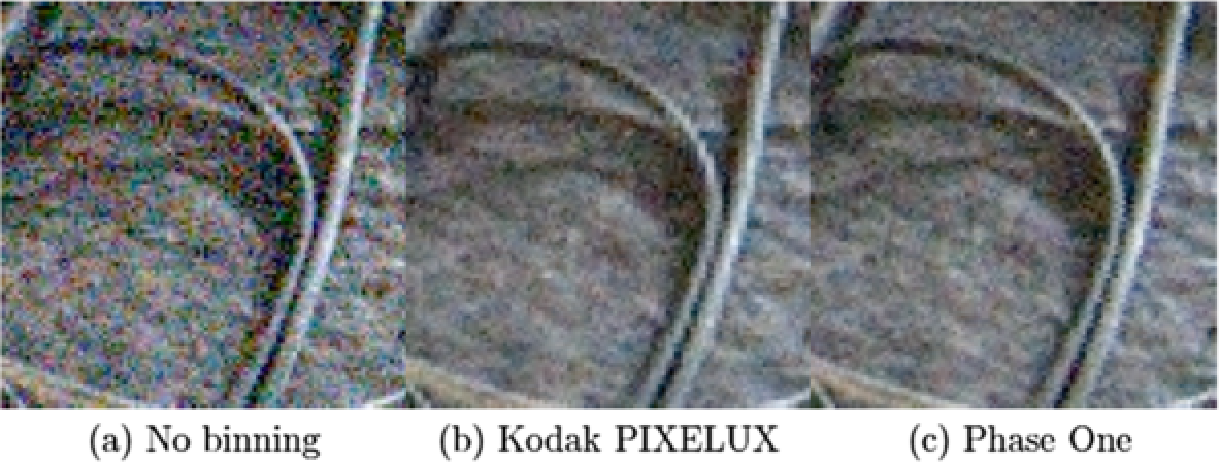
\includegraphics[width=1\linewidth]{images/pixel-binning}
    \caption{Visualisatie van pixel binning~\autocite{Jin2012}}
    \label{fig:pixel-binning}
\end{figure}

%---------- Verwerken van data ---------------------------------------------------------
\subsection{Het verwerken van data uit multimedia}\label{subsec:het-verwerken-van-data}
Om de nauwkeurigheid en snelheid van objectherkenningsalgoritmen zo veel mogelijk te bevorderen worden eerst enkele stappen uitgevoerd ter voorbereiding.
Deze algoritmen kennen immers een langere verwerkingstijd bij grotere bestanden.
Beeldfragmenten ondergaan hiervoor verschillende processen, waaronder het voorgenoemde pixel binningsproces.

\subsubsection{Pixel binning}
Zoals eerder aangehaald kiezen moderne smartphones ervoor om pixels te groeperen in superpixels waarop vervolgens aan pixel binning gedaan wordt.
Het effect hiervan is het verzachten van observeerbare ruis, zoals zichtbaar op afbeelding~\ref{fig:pixel-binning}.
Beelden die genomen zijn in donkere plekken kunnen daarmee een hogere waarneembare beeldkwaliteit krijgen.
Een bijkomend effect van dit proces is de kleinere voetafdruk van de verwerkte beelden doordat er een kleiner aantal pixels overblijven.
In het geval van smartphones wordt vaak gekozen om te binnen richting 12 megapixels, wat tussen de schermresoluties 4K Ultra HD (ongeveer 8 megapixels) en 8K Ultra HD (ongeveer 33 megapixels) ligt.
Deze resoluties worden steeds vaker gebruikt in televisies~\autocite{Statista2024}.

\subsubsection{Transformatie van beelden}
Beeldfragmenten kunnen naast pixel binning op andere manieren bewerkt worden om meer specifieke informatie te benadrukken en op te slaan.
Een voorbeeld hiervan is Fouriertransformatie, zoals beschreven in het onderzoek van~\textcite{Olaoye2024}.
Door middel van deze techniek worden dominante ruimtelijke frequenties benadrukt wat het identificeren van patronen, randen en texturen van beelden mogelijk maakt.
Beelden kunnen daarnaast ook geschaald of gedraaid worden voor geometrische correcties of ter uitlijning van afbeeldingen.
Vervolgens kunnen beelden opgedeeld worden naar gelang de kleur, textuur of randen.

%---------- Toepassen van klassieke algoritmen------------------------------------------
\subsection{Klassieke objectherkenningsalgoritmen}
\label{subsec:klassieke-objectherkenningsalgoritmen}
Na het verwerken van beeldfragmenten komt verdere segmentatie aan bod door middel van klassieke objectherkenningsalgoritmen, wat in vakliteratuur vaak als \textit{feature extraction} vernoemd wordt.
Met behulp van deze algoritmen kunnen we kenmerken van objecten detecteren om vervolgens te classificeren en vergelijken met andere data.
Het verschil van deze algoritmen met moderne objectherkenningstechnieken is het gebrek aan gebruik van machine learning, wat verder aan bod komt in hoofdstuk~\ref{sec:datasets}.

\subsubsection{Histogram van Georiënteerde Gradiënten}
Histogram van Geori\"enteerde Gradi\"enten (HOG) is een simpel algoritme voor kenmerkbeschrijving van objecten voor feature extraction, met als doel om lokale vorm- en textuurinformatie vast te leggen~\autocite{Saher2023}.
Allereerst filtert het HOG-algoritme de kleuren uit de afbeelding zodat enkel de grijswaarden overblijft.
Vervolgens splitst het algoritmede beelden op in kleine overlappende cellen en berekent het de gradi\"enten van elke cel in zowel de horizontale als de verticale richting.
Eveneens legt het de verandering in pixelintensiteit en diens orientatie vast.
Op basis van deze berekeningen kan een histogram van celori\"entaties gegenereerd worden om de lokale gradi\"entverdeling met informatie over randen en textuur weer te geven.

\subsubsection{Schaalinvariante kenmerkentransformatie}
Voor situaties waarin schaal- en rotatie-invariantie belangrijk zijn kan het beter zijn om gebruik te maken van SIFT\@.
\textcite{Tamara2022}~beschrijft Schaalinvariante kenmerkentransformatie (SIFT) als een complexer techniek voor het identificeren van lokale kenmerken in een afbeelding.
\begin{figure}
    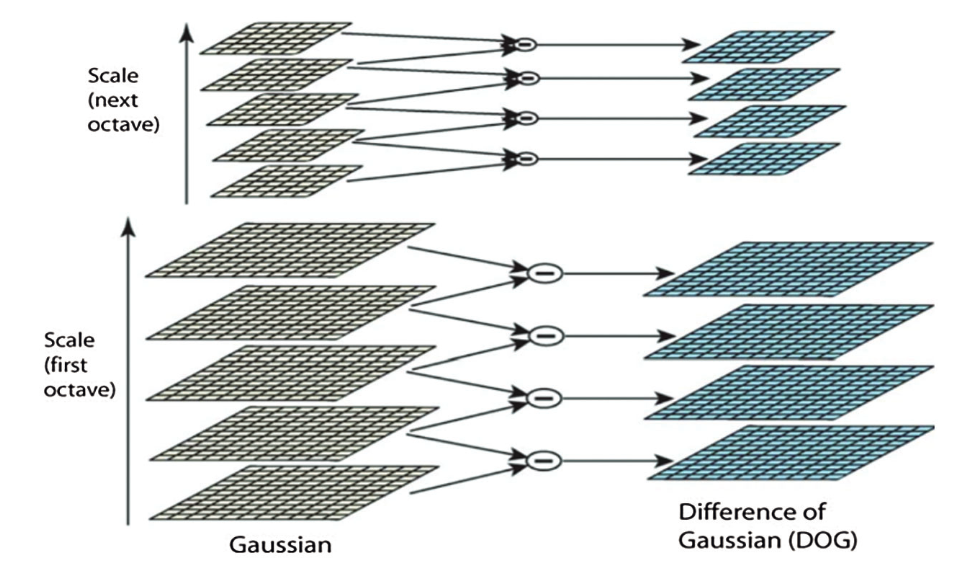
\includegraphics[width=1\linewidth]{images/DoG}
    \caption{Visualisatie van het verschil in Gaussianen~\autocite{Lowe2004}}
    \label{fig:difference-of-gaussian}
\end{figure}
Het eerste deel van dit algoritme bestaat uit het berekenen van de minima en de maxima uit het verschil in Gaussianen (DoG) met verschillende standaardafwijkingen, zoals gevisualiseerd op afbeelding~\ref{fig:difference-of-gaussian}.
Daarna worden uitschieters weggefilterd door middel van een wiskundige Hessische matrix.
Een normalisatie van het aantal kenmerken kan vervolgens behaald worden door een minimum contrast van de verschillende standaardafwijkingen te hanteren.
Het toepassen van ori\"entatietoewijzing verzekert hierbij de eigenschap van rotatie-invariantie.
Uit deze stappen ontstaan enkele SIFT-beschrijvingen die vergelijking met andere afbeeldingen mogelijk maken om te bepalen of ze tot dezelfde categorie horen.
Dit gehele proces kent echter aanzienlijke verwerkingstijd waardoor het gebruik in real-time applicaties beperkt blijft.

\subsubsection{Versnelde robuuste functies}
Een alternatief voor SIFT zijn Versnelde robuuste functies (SURF), een eenvoudiger algoritme met een focus op snelheid over het bereiken van de hoogste nauwkeurigheid~\autocite{Wu2013}.
Het concept van SURF is vergelijkbaar met dat van SIFT, echter maakt SURF gebruik van een andere methode om kenmerkbeschrijvingen te genereren.
In dit algoritme wordt bewust niet gekozen voor DoG en wordt enkel gebruik gemaakt van een Hessische matrix voor de detectie van kenmerken.
Daarnaast maakt het SURF-algoritme gebruik van een eenvoudigere Haar-waveletberekening met de x- en y-richtingen van elk gebied binnen een afbeelding.

%---------- Uitdagingen & beperkingen --------------------------------------------------
\subsection{Uitdagingen en beperkingen}
\label{subsec:uitdagingen-en-beperkingen}
Hoewel er vele mogelijkheden ontstaan door het gebruik van de voorgenoemde voorbeelden van klassieke algoritmen, kent de technologie ook enkele limitaties.
De voorgenoemde algoritmen hebben vaak te maken met moeilijkheden in het detecteren van objecten in complexe situaties~\autocite{Luz2024}.
Variaties in belichting, drukke achtergronden rond objecten en occlusie van objecten verminderen de nauwkeurigheid van deze traditionele algoritmen.
Machine learning kan hierop inspelen door bijkomende attributen toe te wijzen aan objecten.

%%=============================================================================
%% Machine learning
%%=============================================================================
\section{Machine learning}\label{sec:datasets}
Het vorige hoofdstuk definieerde de werking van objectherkenning en diens situering binnen de artifici\"ele intelligentiesector samen met enkele voorbeelden van klassieke algoritmen.
Deze algoritmen kennen enkele beperkingen waar deep learning een antwoord op kan bieden.
De komst van machine learning (ML) kent buiten objectherkenning vele andere toepassingen zoals het ontstaan van grote taalmodellen, wat later aan bod zal komen.

%---------- Hoe werkt machine learning -------------------------------------------------
\subsection{Hoe machine learning en deep learning werkt}
\label{subsec:hoe-deep-learning-werkt}
Net zoals objectherkenning een subset van computer visie is kan deep learning (DL) gezien worden als een subset van machine learning.
Het domein artifici\"ele intelligentie overkoepelt beide vakgebieden.
Concreet maken ML-technieken gebruik van statistieken en optimalisatiemethoden om grote hoeveelheden data te verwerken~\autocite{Pennone2024}.
Hiermee ontstaat de mogelijkheid om uitkomstvoorspellingen te maken op basis van invoer van nieuwe data.
Het algoritme groepeert deze data in subgroepen en classificeert vervolgens elke subgroep.
Daardoor ontstaat de mogelijkheid om onder andere uitkomstvoorspellingen te maken van toekomstige data.
In context van deze paper gaat het daarbij concreet over het classificeren van sportgerelateerde objecten en omgevingen op basis van eerder verwerkte datasets.

%---------- Deep learning in plaats van machine learning -------------------------------
\subsection{Deep learning}
\label{subsec:deep-learning-algoritmen}
Een complexere manier van dataverwerking kan gebeuren aan de hand van DL-algoritmen, een subset van machine learning dat gebruik maakt van neurale netwerken om informatie te verwerken~\autocite{Bozic2024}.
De algoritmen verwerken data door ze op verschillende niveaus te behandelen, in tegenstelling tot simpelere ML-technieken.
In het geval van objectherkenning bestaan de lagere niveaus van een beeldfragment uit randen en vormen, terwijl hogere niveaus de kenmerken uit de lagere niveaus combineren om het object te identificeren.

\subsubsection{Voordelen ten opzichte van machine learning}
Deep learning-technieken produceren vaak betere resultaten ten opzichte van machine learning~\autocite{Ahmed2023}.
Bovendien krijgen ze vaak de voorkeur door volgende redenen:

\paragraph{Structuur van de gebruikte data}
In vele gevallen is de gebruikte data ongestructureerd wegens de verschillende soorten media waarin ze opgeslagen zijn.
De meeste ML-algoritmen hebben moeite met deze data te verwerken waardoor de data vaak onbenut blijft voordat men ervoor kiest om deep learning toe te passen.

\paragraph{Nieuwe kenmerken genereren}
Het belangrijkste voordeel van deep learning vergeleken met andere ML-algoritmen is het vermogen om nieuwe kenmerken te genereren uit de beperkte lijst van kenmerken in de oorspronkelijke dataset.
De DL-algoritmen gebruiken daarbij neurale netwerken doorheen het hele proces waardoor het steeds kan bijleren.
Dit leidt tot een optimalisatie van alle relevante parameters wat uiteindelijk resulteert in een verbeterde nauwkeurigheid.

\paragraph{Zelfstandigheid}
Bovenop het genereren van nieuwe kenmerken kunnen DL-technieken op een zelfstandige basis aan resultaten bekomen.
De algoritmes zoekt daarbij automatisch in de gegevens uit de trainingsdata zonder expliciete instructies te krijgen.
Dit is mogelijk door kenmerken te vergelijken en combineren wat het leerproces bevordert.

\paragraph{Schaalbaar}
Het proces is zeer schaalbaar door de manier waarop het grote hoeveelheden aan data kan verwerken.
Tot gevolg heeft het de mogelijkheid om steeds nauwkeurigere resultaten te produceren bij allerlei verschillende soorten data van verschillende groottes.
Bij grotere datasets ontwikkelt het algoritme een beter begrip voor context en een grotere lijst van functionaliteiten.

\subsubsection{Nadelen van deep learning}
Hoewel DL-technieken vele verbeteringen aanbiedt ten opzichte van machine learning-algoritmen, kent het ook enkele nadelen waardoor het gebruik ervan beperkt wordt bij grotere organisaties:

\paragraph{Hogere rekenkracht}
DL-algoritmen maken gebruik van aanzienlijk grotere hoeveelheden data ten opzichte van ML-technieken.
Dit vergt sterkere computers met meer rekenkracht en opslag.
\paragraph{Afhankelijkheid van data}
Net zoals machine learning-algoritmen kennen DL-technieken een afhankelijkheid van de gebruikte data.
De resultaten van deze technieken zijn afhankelijk van zowel de kwaliteit als de kwantiteit van deze datasets.
Bovendien vereist dit data die gelabeld is, wat kostelijk of in sommige domeinen zelfs onhaalbaar te verkrijgen is~\autocite{Olaoye2024a}.
\paragraph{Complexiteit}
In bepaalde situaties zijn de gebruikte algoritmen complex te interpreteren, deels door de complexiteit van de gebruikte data.
Het is daardoor moeilijker om de beslissingen en resultaten van deze technieken te traceren.
Dit vereist het hertrainen van het algoritme om fouten recht te zetten.

%---------- Deep learning toepassen in objectherkenning---------------------------------
\subsection{Moderne objectherkenningsalgoritmen}
\label{subsec:deep-learning-in-objectherkenning}
Deep learning bouwt verder op klassieke objectdetectiealgoritmen om nauwkeurigheid te bevorderen en de uitdagingen zoals besproken in~\nameref{subsec:uitdagingen-en-beperkingen} te omzeilen.
Door het concept van deep learning ontstaan vele nieuwe algoritmen voor het detecteren van objecten:

\subsubsection{Convolutionele neurale netwerken)}
% Convolutional Neural Networks
Convolutionele neurale netwerken (CNN) hebben het vermogen om automatisch kenmerken te leren uit afbeeldingen aan de hand van convolutielagen~\autocite{Nourmohammadi2024}.
Ze zijn geoptimaliseerd om te werken met ruimtelijke structuren en hebben geen geheugen van voorgaande invoeren.
Ondersteunende vectormachines (SVM) kunnen daarbij gebruikt worden voor classificatietaken zoals objectherkenning.
Beslisbomen kunnen objecten identificeren door middel van een hi\"erarische reeks beslissingen op basis van beschrijvingskenmerken.
Tot slot kunnen K-nabije buren (KNN) objecten identificeren door kenmerken te vergelijken met kenmerken van gelijkaardige objecten in de trainingsdata.

\subsubsection{Terugkerende neurale netwerken}
% Recurrent Neural Networks
Terugkerende neurale netwerken (RNN) daarentegen worden eerder gebruikt voor doeleinden waar context van belang is.
Ze zijn effectief in het onthouden van informatie doorheen verschillende stappen in een sequentie en zijn daarmee nuttig voor spraakherkenning en machinevertaling.
% TODO:
%  populaire datasets, zoals COCO (Common Objects in Context), Pascal VOC (Visual Object Classes), en ImageNet, worden vaak gebruikt voor het trainen en evalueren van objectherkenningsalgoritmen.

%%=============================================================================
%% Generatieve AI
%%=============================================================================
\section{De werking van grote taalmodellen}
\label{sec:ls-artificiele-intelligentie}
Met een kennis over de manier waarop datasets gebruikt worden in machine learning kan tot slot het concept van generatieve AI verklaard worden.
Generatieve AI verwijst hierbij naar de technologie van kunstmatige intelligentie om nieuwe gegevens voor te stellen op basis van trainingsdata~\autocite{Gupta2023}.
Een voorbeeld hiervan is ChatGPT, een AI-chatbot die beschikbaar gesteld wordt door OpenAI\@.
Gebruikers hebben daarbij de mogelijkheid om teksten te laten vertalen, broncode voor software te genereren of gedichten op te stellen.
Dit alles gebeurt in een tekstgebaseerde interactieomgeving, waarbij gebruikers met de applicatie praten alsof ze communiceren in een chatapplicatie.

\subsection{Vooruitgang van taalmodellen}
\label{subsec:vooruitgang-van-taalmodellen}
\textcite{OpenAI2023}, een onderzoeksinstituut met het doel om veilige en nuttige algemene artifici\"ele intelligentie te ontwikkelen, beschrijft gunstige resultaten in haar technisch rapport over de nieuwere iteraties van het GPT-model met het trainen van steeds grotere datasets.
De voorgenoemde generatieve AI-toepassing ChatGPT maakt daarbij gebruik van versie 3.5 van het model om verzoeken van gebruikers te vervullen.
In het rapport haalt OpenAI aan dat versie 4 van haar GPT-model een score behaalt die in de top tien percent van de testnemers valt bij het afnemen van een gesimuleerde balie-examen.
Versie 3.5 daarentegen scoort bij de laagste tien percent, wat een opmerkzame evolutie is.
Het rapport geeft verschillende vergelijkbare resultaten weer, een daarvan is zichtbaar op afbeelding~\ref{fig:gpt3.5-versus-4} waarbij beide modellen enkele academische en professionele examens afleggen.
\begin{figure}
    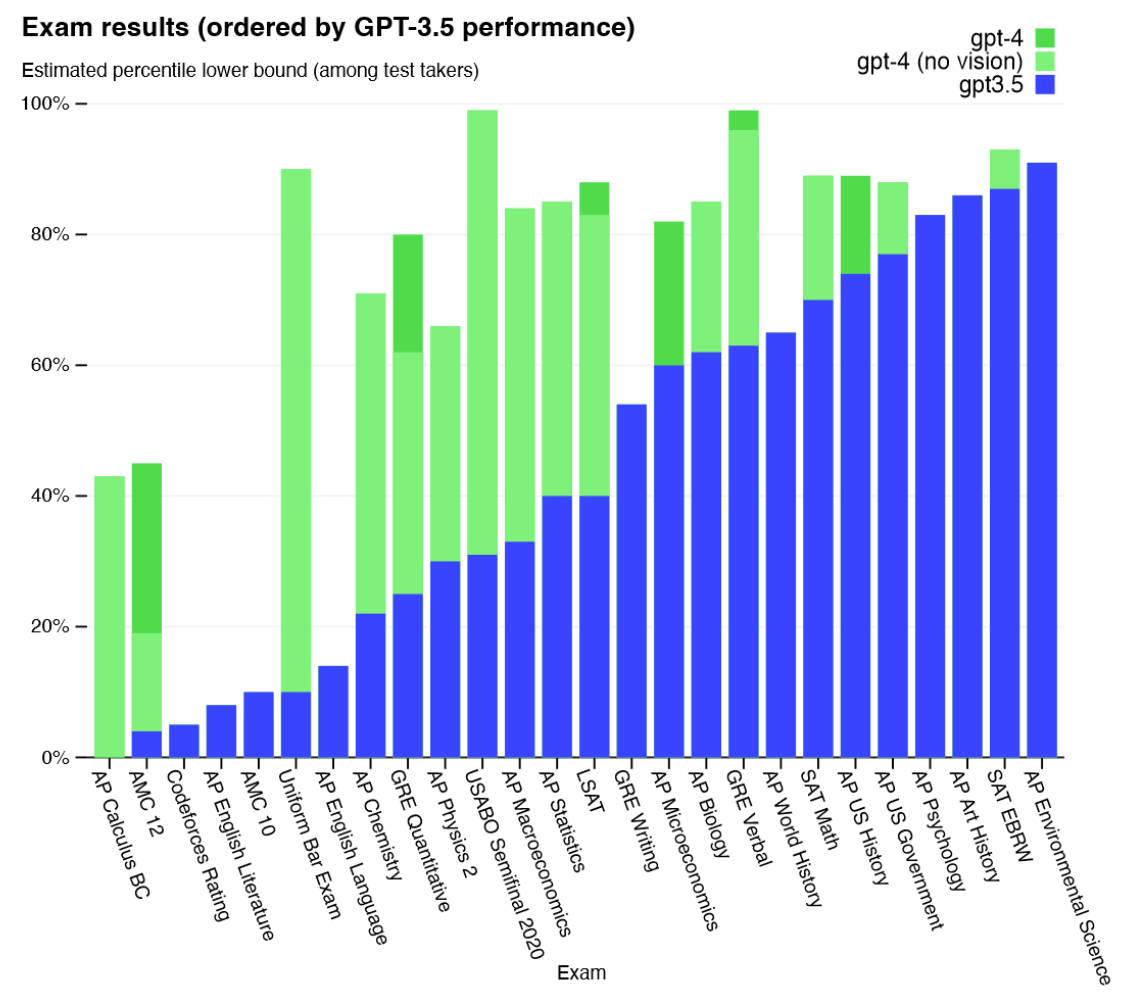
\includegraphics[scale=0.5]{images/gpt35-vs-4-exam-results}
    \caption{Vergelijking tussen GPT 3.5 en GPT 4 bij het afleggen van verschillende academische en professionele examens. Bijkomende computer visie mogelijkheden helpen GPT-4 om betere resultaten te halen~\autocite{OpenAI2023}}.
    \label{fig:gpt3.5-versus-4}
\end{figure}

\subsection{Versterkingsleren via menselijke feedback}
\label{subsec:versterkingsleren-via-menselijke-feedback}
Versterkingsleren via menselijke feedback (RLHF) heeft de mogelijkheid om de nauwkeurigheid van modellen te bevorderen na de initi\"ele dataset verwerking.
RLHF is een voorbeeld van versterkend leren waarbij ML-algoritmen geoptimaliseerd worden om nauwkeurigere resultaten te produceren die beter afgestemd zijn op specifieke verwachtingen~\autocite{Balakrishnan2024}.
Dit proces vindt zich plaats na een dataset verwerkt is en er een AI-model tot stand is gekomen dat capabel is om taken uit te voeren.
Met RLHF kunnen vakexperts of data ingenieurs de prestaties van het model beoordelen en corrigerende feedback geven.
Deze feedback zorgt ervoor dat het model bijgestuurd wordt om specifiekere resultaten weer te geven.

\subsection{Generatieve AI en deep learning}
\label{subsec:generatieve-ai-en-deep-learning}
Generatieve AI bouwt verder op het concept van deep learning om grote taalmodellen (LLM) te ontwikkelen~\autocite{Shen2024}.
LLM's hebben door middel van deep learning de mogelijkheid om natuurlijke taal te begrijpen en suggesties te genereren.
Deze AI-modellen richten zich specifiek op het verwerken en genereren van tekstuele data.

\subsubsection{Tokens binnen een verzoek aan een taalmodel}
\textcite{Cope2023} beschrijven tokens in context van grote taalmodellen als volgt:
``De elementaire eenheid van analyse in de LLM is het token.
Soms is dit een woord, maar in het geval van woorden met samengestelde betekenissen, kan een token minder zijn dan een woord.
Gereduceerd tot binaire notatie, abstraheert de machine tokens in een identieke, en voor de doeleinden van zijn analyse, betekenisloze vorm.
Ze variëren alleen in het gekwantificeerde gewicht van hun nabijheid tot andere tokens(vectoren) in geschreven tekstcorpora.''
Hiermee ontstaat de stelling dat tokens de maateenheid voor verzoeken aan taalmodellen vormen.
Dit kan doorgetrokken worden voor multimedia zoals afbeeldingen en geluidsfragmenten, door de grotere inhoud aan data bestaan deze logischerwijs uit grotere hoeveelheden tokens.